\documentclass{beamer}
\beamertemplatenavigationsymbolsempty
\usecolortheme{beaver}
\setbeamertemplate{blocks}[rounded=true, shadow=true]
\setbeamertemplate{footline}[page number]
%
\usepackage{hyperref}
\usepackage[utf8]{inputenc}
\usepackage[english,russian]{babel}
\usepackage{amssymb,amsfonts,amsmath,mathtext}
\usepackage{subfig}
\usepackage[all]{xy} % xy package for diagrams
\usepackage{array}
\usepackage{multicol} % many columns in slide
\usepackage{hyperref} % urls
\usepackage{hhline} %tables
\usepackage{comment} %comments
% Your figures are here:
\graphicspath{ {../figures/} }

\newcommand{\btVFill}{\vskip0pt plus 1filll}
\newcommand{\secref}[1]{\autoref{#1}. \nameref{#1}}
%----------------------------------------------------------------------------------------------------------

\title[\hbox to 56mm{Детекция зависимостей во временных рядах}]{Детекция зависимостей во временных рядах}
\author[И. М. Латыпов]{Ильгам Магданович Латыпов}
\institute[]{Московский физико-технический институт}
\date{\footnotesize
	\par\smallskip\emph{Курс:} Моя первая научная статья
	\par\smallskip\emph{Эксперт:} В. В. Стрижов
	\par\smallskip\emph{Консультант:} Э. Владимиров
	\par\bigskip\small 11\;апреля\;2023\,г.}

%----------------------------------------------------------------------------------------------------------
\begin{document}
	%----------------------------------------------------------------------------------------------------------
	
	\begin{frame}
		
		%\thispagestyle{empty}
		\maketitle
		
	\end{frame}
	
	%-----------------------------------------------------------------------------------------------------
	
	\begin{frame}{Цели исследования}
		
		\textbf{Задача}: Детектирование причинно следственных взаимосвязей между временными рядами.
		
		\textbf{Проблема}: Не существует методов которые точно выявляют факто причино-следственной зависимости между временными рядами. А те которые существуют направлены на работу с одномерными временными рядами.
		
		\bigskip
		
		\textbf{Цель}: Разработать параметрический метод для решения поставленной задачи в многомерном случае.
		
		\bigskip
		\textbf{Идея}: Параметрический метод на основе метода сходящегося перекрестного отображения.
	\end{frame}
	
	%-----------------------------------------------------------------------------------------------------
	
	\begin{frame}{Литература}
		\textbf{1.} James M. McCracken and Robert S. Weigel. Convergent cross-mapping and pairwise
		asymmetric inference. Physical Review E, 90(6), dec 2014
		
		\textbf{2.} В.В. Стрижов К.Р. Усманова. МОДЕЛИ ОБНАРУЖЕНИЯ ЗАВИСИМОСТЕЙВО
		ВРЕМЕННЫХ РЯДАХ В ЗАДАЧАХ ПОСТРОЕНИЯПРОГНОСТИЧЕСКИХ МОДЕЛЕЙ. «Системы и средства информатики», 2018
		
		\textbf{3.} V. V. Strijov A. V. Grabovoy. Quasi-periodic time series clustering for human activity recognition. http://strijov.com/papers/Grabovoy2019QuasiPeriodicTimeSeries.pdf, 2018.
		
	\end{frame}
	
	%-----------------------------------------------------------------------------------------------------
	
	\begin{frame}{Метод сходящегося перекрестного отображения}
		Траекторная матрица
		$$
		\mathbf{H}_{x} =
		\left( {\begin{array}{ccccc}
				x_1 & x_2 & ... & x_{L-1} & x_L\\
				x_2 & x_3 & ... & x_{L} & x_{L +1}\\
				... & ... & ... & ...   & ... \\
				x_{N-L+1} & x_{N-L +2} & ... & x_{N-1} & x_N\\
		\end{array} } \right) = 
		\left( {\begin{array}{c}
				\mathbf{x_L}\\
				\mathbf{x_{L + 1}}\\
				...         \\
				\mathbf{x_N}\\
		\end{array} } \right)
		$$
		
		Отображение $\phi$  между траекторными пространствами
		
		$$
		\phi: x^0 \rightarrow \hat y^0 \sum^k_{i = 1} w_iy^{t_i}, \qquad w_i = \frac{u^i}{\sum_i u_i}, \qquad u_i = \exp(-\frac{\|x^0 - x^{t_i}\|_2}{\|x^0 - x^{t_k}с\|_2})
		$$
		
		Метрика связанности временных рядов
		
		$$
		Score_{X\rightarrow Y} Corr(\phi(\mathbf{x}), \mathbf{y})
		$$
	\end{frame}
	
	%----------------------------------------------------------------------------------------------------------
	
	\begin{frame}{Предлагаемый метод}
		\textbf{Идея}: Параметризуем способ построения траекторного пространства в методе сходящегося перекрестного отображения.
		
		\textbf{Нововведение}:Для этого используется модель пространства состояний.
		
		\textbf{Как работает}:  Совместно с временным рядом рассматривается вектор скрытых состояний $\mathbf{u}$, который эволюционирует с исходной системой
		
		% \begin{equation}
			$$
			\begin{split}
				\mathbf{u_0} = f(\mathbf{x_0}) \\ 
				\mathbf{u_{k + 1}} = \psi(\mathbf{u_k}, \mathbf{x_k}) 
			\end{split}
			$$
			% \end{equation}
		
	\end{frame}
	
	%----------------------------------------------------------------------------------------------------------
	\begin{frame}{Эксперименты}
		\textbf{Постановка}: Рассмотим в качестве $\psi$ ГНС ODE-RNN^{\hyperref[paper]{1}}
		
		Траектории пары рядов в траекторном пространстве при применении разных методов
		
		\begin{columns}
			\begin{column}{0.1\textwidth}
				
				CCM
				\newline
				\newline
				\newline
				
				
				предлагаемый
				
			\end{column}
			
			\begin{column}{0.8\textwidth}
				
				\begin{figure}
					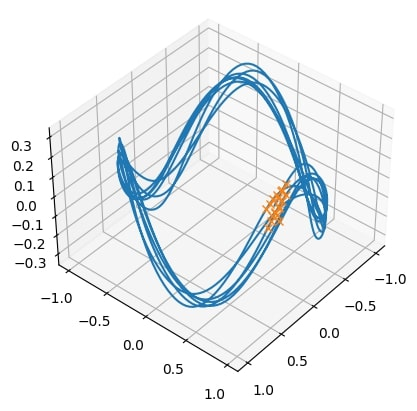
\includegraphics[width = 0.3\textwidth]{images/trajectory_CCM.jpg}
					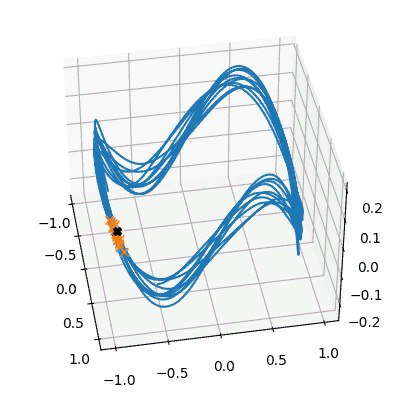
\includegraphics[width = 0.3\textwidth]{images/trajectory_CCM_right.jpg}  
					\\[\smallskipamount]
					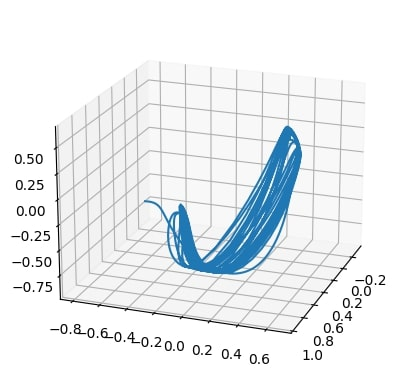
\includegraphics[width = 0.3\textwidth]{images/trajectory_left.jpg}
					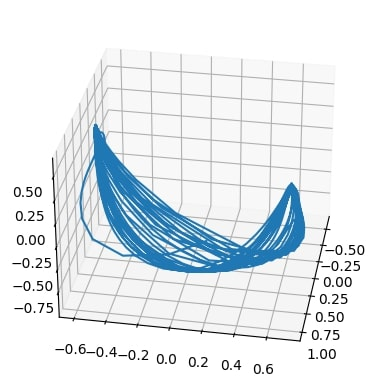
\includegraphics[width = 0.3\textwidth]{images/trajectory_right.jpg}
				\end{figure}
				
			\end{column}
		\end{columns} 
		
		
		\btVFill
		\hline
		\font\myfont=cmr12 at 6pt
		\label{paper}
		\myfont Rubanova, Yulia / Chen, Ricky T. Q. / Duvenaud, David | Latent ODEs for Irregularly-Sampled Time Series | 2019
	\end{frame}
	
	%----------------------------------------------------------------------------------------------------------
	
	
	\begin{frame}{Результаты экспериментов}
		
		Так как траектории скрытых состояний представляют собой периодическую структуру можем применять к ним метод сходящегося перекрестного отображения
		
		
		----------------------------------------------------
		
		красивый график
		
		==========================
	\end{frame}
	
	%----------------------------------------------------------------------------------------------------------
	
	\begin{frame}{Промежуточные выводы}
		\begin{itemize}
			\item Разработан метод для выявления зависимостей в многомерных временных рядах.
			\item не исследованы границы применимости метода.
		\end{itemize}
	\end{frame}
	
	%----------------------------------------------------------------------------------------------------------
\end{document}